\documentclass[a4paper,11pt,dvipdfmx]{ujarticle}
% パッケージ
\usepackage{graphicx}
\usepackage{url}
% レイアウト指定を記述したファイルの読み込み
\input{layout}

% タイトルと氏名を変更せよ．
\title{日本におけるデジタル化の状況}
\author{G684292026 江端 希未煌}

\begin{document}

\maketitle %ここにタイトルが入る

% ここから本文
\section{デジタル競争ランキング}% 節見出し: \section{}
% を使う
国際経営開発研究所(IMD)の調査\cite{imd}によると,
日本のデジタル競争力のランキングは図\ref{fig:ranking}に示すよに,
調査対象の64ヵ国中,
総合で28位,
知識分野で25位となっている.

% 本文(1)
%  参考文献の参照: \cite{}
%  図番号の参照： \ref{}
% を使う
% 文献データベースのキーワードは oecd と imd
% になっている．
\begin{figure}[htbp]
    \centering
    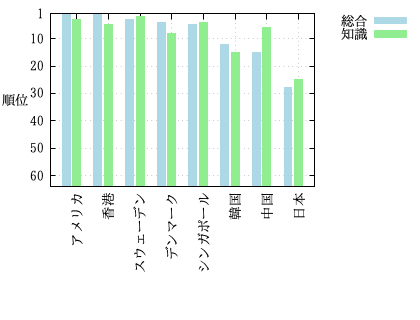
\includegraphics[width=0.7\linewidth]{fig32.png}
    \caption{デジタル競争力ランキング(64ヵ国中)}\label{fig:ranking}

\end{figure}

% 図の挿入
% を
% \begin{figure}[htbp]
% \end{figure}
% で囲み
% \caption{}
% で図のタイトルを入れる．
% \label{}
% を使って図番号が参照できるようにする
% また，
% \centering
% で図が中央に来るようにする

% ーーー
\newpage
\section{ブロードバンド}% 節見出し(2)

% 本文(2)
OECDによるブロードバンド回線の普及に関する調査\cite{oecd}による,表\ref{tab:broadband}に示すように,
日本における100人あたりのモバイルブロードバンドの加入者数は190.5で、第1位になっている.
2位はエストニアで,3位米国と続く.

% 表の挿入
\begin{table}[htbp]
    \centering
    \caption{モバイルブロードバンドの加入者数 (100人あたり) }
    \label{tab:broadband}
    \begin{tabular}{|c|l|r|}
        \hline
        順位 & 国名 & 加入者数 \\ \hline
        1位 & 日本 & 190.5 \\
        2位 & エストニア & 179.9 \\
        3位 & 米国 & 169.0 \\
        4位 & フィンランド & 157.0 \\
        5位 & デンマーク & 141.7 \\
        6位 & ラトビア & 141.6\\
        7位 & イスラエル & 139.9\\
        8位 & オランダ & 133.3\\
        9位 & ポーランド & 131.3\\
        10位 & スウェーデン & 127.2\\ \hline
    \end{tabular}
\end{table}
% \end{tabular}    
% による表の記述を 
% \begin{table}[htbp]
% \end{table}
% で囲み
% \caption{}
% で表のタイトルを入れる．
% \label{}
% を使って表番号が参照できるようにする
% また，
% \centering
% で表が中央に来るようにする

% ーーー
\section{考察}% 見出し(3)
\begin{itemize}
    \item 日本はモバイルブロードバンドの普及率（インフラ）において世界的トップクラスである.
    \item デジタル競争力ランキングでは28位と、通信環境の良さを十分に活かしきれていない.
    \item 優れたインフラ（ハードウェア）を活用できるデジタル人材の育成や、組織の変革（ソフトウェアや知識面）の強化が課題であると考える.
\end{itemize}

% ここに参考文献が入る
%
\bibliographystyle{junsrt}
\bibliography{exercise.bib}

\end{document}